%versi 2 (8-10-2016)
\chapter{Landasan Teori}
\label{chap:teori}
Pada bab ini dijelaskan dasar-dasar teori mengenai \textit{Wireless Sensor Network}, transfer data pada wireless sensor network, prinsip \textit{reliable data transfer} pada Wireless Sensor Network, dan pengembaganan pemrograman pada WSN.

\section{Wireless Sensor Network}
\label{sec:wsn}
\textit{Wireless Sensor Network} merupakan jaringan nirkabel yang terdiri dari sekumpulan \textit{sensor node} yang diletakan pada suatu tempat dan memiliki kemampuan untuk mengukur kondisi lingkungan sekitar(\textit{sensing}), komputasi dan dilengkapi dengan alat komunikasi \textit{wireless} untuk komunikasi antar \textit{sensor node}. Sensor ini akan mengumpulkan data dari kondisi lingkungannya, seperti: cahaya, suara, kelembapan, getaran, gerakan, temperatur, tekanan udara, kualitas air, komposisi tanah, dan lain-lain. Data ini kemudian dikirimkan ke \textit{sensor node} tetangganya hingga sampai ke \textit{base station} sebagai pusat untuk dikelola.

\subsection{Penerapan Wireless Sensor Network}
Pada awalnya \textit{sensor network} (jaringan sensor) digunakan dalam teknologi militer untuk mendeteksi musuh di laut dan di darat. Semakin lama sensor node ini banyak dikembangkan untuk membantu berbagai bidang kehidupan manusia. Pemanfaatan Wireless Sensor Network pada kehidupan manusia dapat dilihat pada ilustrasi Gambar~\ref{fig:smartworld}. Berikut adalah beberapa penerapan wireless sensor network pada berbagai bidang kehidupan manusia:
\begin{itemize}
\item Bidang militer\\
\textit{Wireless Sensor Network} digunakan sebagai bagian dari komunikasi pada bidang militer dan deteksi target atau musuh.

\item Monitoring area\\
Pada \textit{monitoring area}, \textit{sensor node} akan disebar pada suatu tempat yang akan di monitoring. Saat \textit{sensor node} mendeteksi kejadian(panas, tekanan, dan lain-lain) pada suatu tempat, data akan dikirimkan ke \textit{base station} untuk ditentukan tindakan selanjutnya.

\item Transportasi\\
Pada bidang transportasi \textit{Wireless Sensor Network} digunakan untuk mendeteksi lalu lintas secara aktual yang nantinya akan disampaikan kepada pengendara tentang kejadian di depan mereka seperti kemacetan lalu lintas. 

\item Kesehatan\\
Beberapa aplikasi kesehatan seperti membantu pada disabilitas, monitoring pasien, diagnosis, pengaturan penggunaan obat, dan pelacakan dokter dan pasien di rumah sakit.

\item Deteksi lingkungan\\
Deteksi lingkungan yang dapat dilakuan antara lain deteksi gunung berapi, polusi udara, kebakaran hutan, efek rumah kaca, dan deteksi longsor.

\item Monitoring struktur\\
\textit{Wireless Sensor Network} dapat melakukan deteksi pergerakan bangunan dan infrastruktur seperti jembatan, \textit{flyover}, terowongan dan fasilitas lain tanpa mengeluarkan biaya untuk melakukan dektesi manual dengan mendatangi tempatnya secara langsung.

\item Bidang pertanian\\
Pada bidang pertanian dapat membantu pengelola pertanian untuk melihat penggunaan air dalam irigasi dan mengelola buangan pertanian mereka.
\end{itemize}

\begin{figure} [H]
	\centering  
	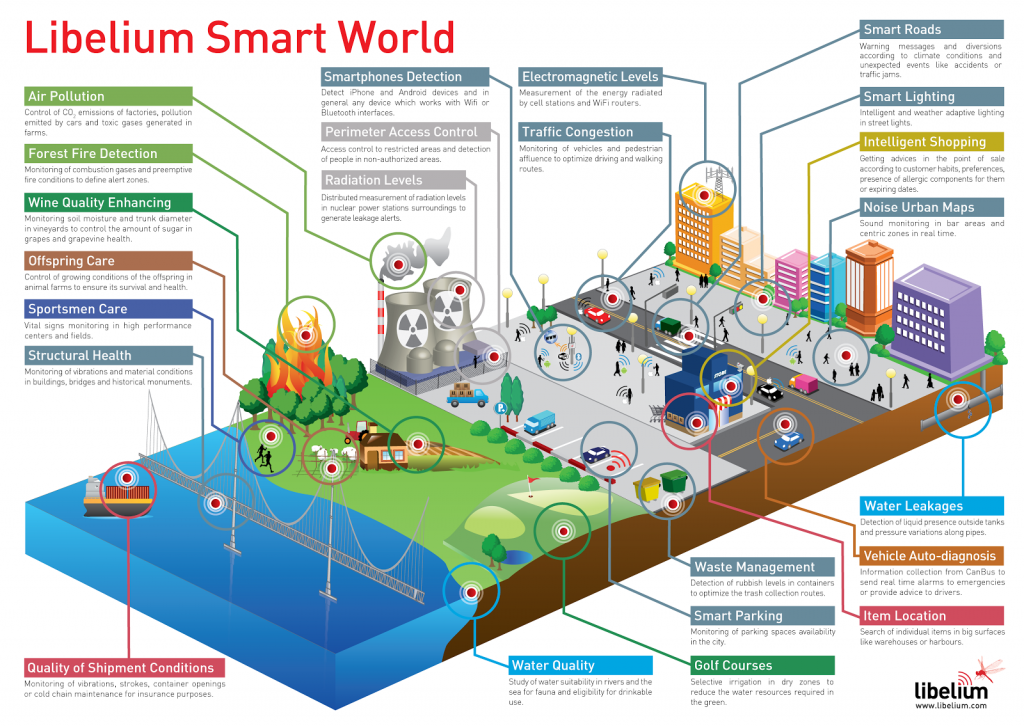
\includegraphics[scale=0.3]{libelium_smart_world}  
	\caption[Ilustrasi Pemanfaatan \textit{Wireless Sensor Network}]{Ilustrasi Pemanfaatan \textit{Wireless Sensor Network}} 
	\label{fig:smartworld} 
\end{figure} 

\subsection{Sensor Node}
%ganti gambar strutur sensor node
\subsubsection{Struktur Sensor Node}
Setiap sensor node memiliki kemampuan deteksi, komputasi dan komunikasi. Sensor node memiliki lima komponen utama yaitu \textit{controller}, \textit{memory}, \textit{sensor and actuator}, \textit{communication device}, dan \textit{power supply}, (Gambar~\ref{fig:structure_sensor_node}). Semua komponen akan bekerja secara seimbang dalam melakukan sensing, komputasi, komunikasi, dan menjaga penggunaan energi seminimal mungkin. 

\begin{figure} [H]
	\centering  
	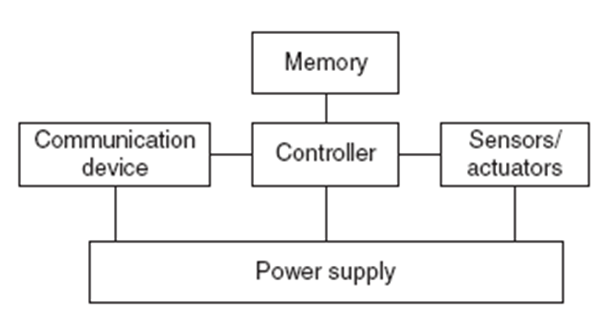
\includegraphics[scale=1]{structure_sensor_node}  
	\caption[Struktur Sensor Node]{Struktur Sensor Node} 
	\label{fig:structure_sensor_node} 
\end{figure} 

\subsubsection{Controller}
Controller adalah inti utama pada sensor node. Controller mengumpulkan data dari sensor dan memproses data tersebut hingga menentukan kapan dan kemana data tersebut dikirim. Controller menerima data dari sensor node lain. Pada controller biasanya terdapat microcontroller atau microprocessor yang mengatur dan melakukan komputasi data dari sensor node. Microcontroller ini juga dapat mengurangi penggunaan energi dengan masuk ke sleep states yang berarti hanya bagian dari controller saja yang aktif.

Beberapa microcontroller yang digunakan dalam Wireless Sensor Node:
\begin{itemize}
	\item Intel StrongARM (32-bit RISC, up to 206 MHz)
	\item Texas Instrument MSP 430 (16-bit RISC, up to 4 MHz,RAM 2-10 kB)
	\item Atmel Atmega 128L (8-bit)
\end{itemize}

\subsubsection{Memory}
Random Access Memory (RAM) digunakan untuk menyimpan sementara hasil yang didapat dari sensor. RAM juga menyimpan sementara paket dari sensor node lain. Saat power supply terjadi masalah maka data pada RAM ini akan hilang. Ini merupakan salah satu kekurangan dari penggunaan RAM. Maka untuk menyimpan kode program digunakanlah Read Only Memory (ROM). ROM ini biasa disebut Electrically Erasable Programmable Read-Only Memory (EEPROM) atau Flash Memory. Flash memory dapat menyimpan data jika suatu saat data pada RAM hilang atau energi sudah habis (intermediate storage).

\subsubsection{Communication Device}
\textit{Communication Device} digunakan untuk bertukar data antar sensor node. Pada aplikasi Wireless Sensor Network, Radio Frequency(RF)-based adalah media komunikasi yang paling relevan saat ini. RF-based mendukung jangkauan yang jauh, data rate yang tinggi, dapat menerima error rate pada penggunaan energi, dan tidak perlu saling mengetahui posisi antara penerima dan pengirim.

Pada sensor node dibutuhkan transmitter dan receiver untuk menerima dan mengirim data. Kedua hal ini dapat digabung dan disebut dengan transceiver. Tugas transceiver adalah mengubah stream bit dari microcontroller dan mengubahnya menjadi gelombang radio. Selain itu transceiver juga dapat mengubah gelombang radio menjadi stream bit.

\subsubsection{Sensor dan Actuator}
Sensor dan Actuator adalah hal yang penting pada Wireless Sensor Network. Tanpa sensor dan actuator maka sensor node tidak berguna dan tidak dapat digunakan. Tabel~\ref{tab:sensor} adalah jenis - jenis sensor yang dapat dimiliki \textit{sensor node}. Sensor dikategorikan menjadi tiga:
\begin{enumerate}
	\item \textbf{Passive, omnidirectional sensors} Sensor ini dapat mengukur kualitas dari lingkungan fisik tempat sensor node tersebut tanpa mengubah lingkungannya. Beberapa sensor dikategori ini \textit{self-powered}, sensor mendapatkan energi yang mereka butuhkan dari lingkungannya. Energi ini digunakan untuk memperkuat sinyal analog. \textit{Omnidirectional} berarti tidak ada arah pada sensor ini. Sensor akan memancarkan sinyalnya ke segala arah. Contoh sensor ini adalah termometer, sensor cahaya, sensor getaran, mikrofon, sensor kelembapan, sensor tekanan udara, sensor deteksi asap, dan lain-lain.
	\item \textbf{Passive, narrow-beam sensors} Sensor ini memiliki sifat yang sama yaitu pasif, tidak mengubah lingkungannya. Sensor ini dapat melakukan gerakan dan memiliki arah atau daerah pengukuran. Contoh dari sensor ini adalah kamera yang bisa mengukur sesuai dengan arah yang dituju.
	\item \textbf{Active Sensor} Sensor ini aktif dalam memeriksa lingkungannya. Contoh dari sensor ini adalah sonar, radar atau sensor seismik. Sensor ini menghasilkan gelombang dengan ledakan kecil untuk melakukan deteksi.
\end{enumerate}

Actuator jumlahnya beragam seperti sensor. Actuator adalah penerima sinyal dan yang mengubahnya ke aksi fisik. Salah satu aktuator adalah LED, yang mengubah listrik menjadi cahaya. Motor (electrical motor) juga mengubah listrik menjadi gerakan.

\begin{table} [H]
	\centering 
	\caption{Jenis - jenis sensor yang dapat dimiliki sensor node}
	\label{tab:sensor}
	\begin{tabular}{|c|c|c|}
		\toprule
		Sensor & Sense Event & Remark\\

		\midrule
		Accelerometer & & \\
		Acoustic emission sensor &  & \\
		Acoustic sensor &  & \\
		Capacitance sensor &  & \\
		ECG &  & \\
		EEG &  & \\
		EMG &  & \\
		Electrical/electromagnetic sensor &  & \\
		Gyroscope &  & \\
		Humidity Sensor &  & \\
		Infrasonic sensor &  & \\
		Magnetic sensor &  & \\
		Oximeter &  & \\
		pH sensor &  & \\
		Photo acoustic spectroscopy &  & \\
		Piezoelectric cylinder  &  & \\
		Soil moisture sensor &  & \\
		Temperature sensor &  & \\
		Barometer sensor &  & \\
		Passive infrared sensor &  & \\
		Seismic sensor &  & \\
		Oxygen sensor &  & \\
		Blood flow sensor &  & \\

		\bottomrule
		
	\end{tabular} 
\end{table}

\subsubsection{Power Supply}
Power supply atau sumber energi pada Wireless Sensor Network bisa berasal dari dua cara yaitu \textbf{\textit{storing energy}} dan \textbf{\textit{energy scavenging}}. \textit{Storing energy} adalah dengan menggunakan baterai sebagai sumber energinya. Baterai yang digunakan dapat diisi ulang maupun yang tidak dapat diisi ulang. \textit{Energy scavenging} digunakan saat membuat Wireless Sensor Network yang akan digunakan dalam waktu yang lama. Dibutuhkan energi yang bisa dikatakan tidak terbatas. Salah satu cara \textit{energy scavenging} adalah \textit{Photovoltaics}. \textit{photovoltaics} dapat disebut juga \textit{solar cell} yang memanfaatkan cahaya matahari dan mengubahnya menjadi energi sebagai pembangkit daya. Cara lain yang bisa digunakan adalah pemanfaatan angin dan air untuk mengerakan kincir atau turbin yang akan menghasilkan listrik dan digunakan sebagai sumber energi pada sensor node.

\subsubsection{Macam - Macam Node Sensor pada WSN}

\subsection{Arsitektur dan Topologi Wireless Sensor Network}
Pada \textit{Wireless Sensor Network} biasanya akan terdapat banyak \textit{sensor node} yang disebar pada suatu tempat. Terdapat satu atau lebih \textit{sink node} atau \textit{base station} dalam area sensing tersebut (Gambar~\ref{fig:arsitektur}). \textit{sink node} atau \textit{base station} adalah sensor node yang bertugas untuk mendapatkan data dari \textit{sensor node} lain. Dalam membuat \textit{Wireless Sensor Network} perlu diperhatikan arsitektur dan topologi yang akan digunakan. Tidak semua topologi jaringan komputer dapat digunakan untuk \textit{Wireless Sensor Network}. 

Ada banyak topologi pada jaringan sensor (\textit{sensor network}). Pada jaringan sensor dengan menggunakan kabel topologi yang sering digunakan adalah topologi \textit{star}, \textit{line}, atau \textit{bus}. Sedangkan pada jaringan sensor tanpa kabel (WSN) topologi yang biasa digunakan adalah \textit{star}, \textit{tree}, atau \textit{mesh}. 

\subsubsection{Topologi Bus}
Topologi bus seperti pada Gambar~\ref{fig:bus} akan terdiri dari node-node dan sebuah jalur. Setiap node akan terhubung dengan jalur yang sama. Untuk mengirim data atau komunikasi akan dilakukan bergantian antar node. Kekurangan dari topologi bus ini adalah jika suatu saat jalur / bus ini mengalami kerusakan maka setiap node tidak dapat berkomunikasi lagi.
\begin{figure} [H]
	\centering  
	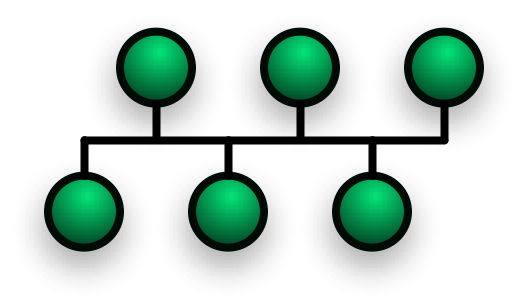
\includegraphics[scale=1]{bus}  
	\caption[Topologi Bus]{Topologi Bus} 
	\label{fig:bus} 
\end{figure} 

\subsubsection{Topologi Ring}
Pada topologi ring node akan disusun dengan bentuk melingkar (Gambar~\ref{fig:ring}). Setiap node akan terkoneksi dengan dua node lain. Transfer data terjadi dengan cara data akan berjalan dari satu node ke node lain mengikuti jalur melingkar tersebut hingga menemukan node tujuan yang tepat. Topologi ini mudah untuk diimplementasikan tapi kekurangan dari topologi ring adalah saat ada node yang rusak maka perlu biaya lebih untuk memperbaikinya. Biasanya node untuk menangani kegagalan komunikasi akibat node yang rusak, akan di atur komunikasi node tidak hanya satu arah tetapi dapat ke arah sebaliknya.
\begin{figure} [H]
	\centering  
	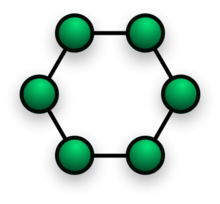
\includegraphics[scale=1]{ring}  
	\caption[Topologi Ring]{Topologi Ring} 
	\label{fig:ring} 
\end{figure} 

\subsubsection{Topologi Star}
Topologi star terdiri dari satu node yang berada di tengah biasanya berupa hub atau switch seperti pada Gambar~\ref{fig:star}. Setiap node akan terkoneksi dengan node yang berada di tengah ini. Saat node akan berkomunikasi dengan node lain, node tersebut harus mengirimkan data tersebut ke node yang ada ditengah dahulu dan node yang ditengah ini akan meneruskan data tersebut ke node tujuan. Yang paling penting pada topologi ini adalah node yang berada di tengah, karena semua komunikasi harus melalui node tersebut. Jika node tengah mengalami kerusakan maka tidak akan terjadi komunikasi antar node pada jaringan tersebut.
\begin{figure} [H]
	\centering  
	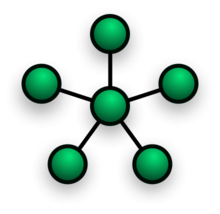
\includegraphics[scale=1]{star}  
	\caption[Topologi Star]{Topologi Star} 
	\label{fig:star} 
\end{figure} 

\subsubsection{Topologi Tree}
Pada topologi tree node-node akan disusun secara hierarki dengan satu node yang berada pada level paling atas sebagai \textit{root node} (Gambar~\ref{fig:tree}). \textit{Root node} akan terhubung dengan satu atau lebih node level dibawahnya. Dengan topologi tree lebih mudah untuk melakukan identifikasi dan meminimalisir kesalahan, namun jika tree sudah sangat besar / level tree sudah sangat banyak maka akan sulit untuk mengaturnya.
\begin{figure} [H]
	\centering  
	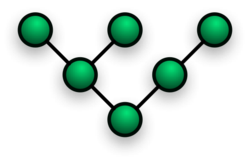
\includegraphics[scale=1]{tree}  
	\caption[Topologi Tree]{Topologi Tree} 
	\label{fig:tree} 
\end{figure} 

\subsubsection{Topologi Mesh}
Topologi mesh dibagi menjadi dua yaitu partially connected mesh dan fully connected mesh. Pada partially connected mesh (Gambar~\ref{fig:mesh_partial}), node akan terhubung dengan lebih dari satu node. Pada fully connected mesh (Gambar~\ref{fig:mesh_fully}), setiap node akan terhubung dengan semua node lain pada jaringan tersebut
\begin{figure} [H]
	\centering  
	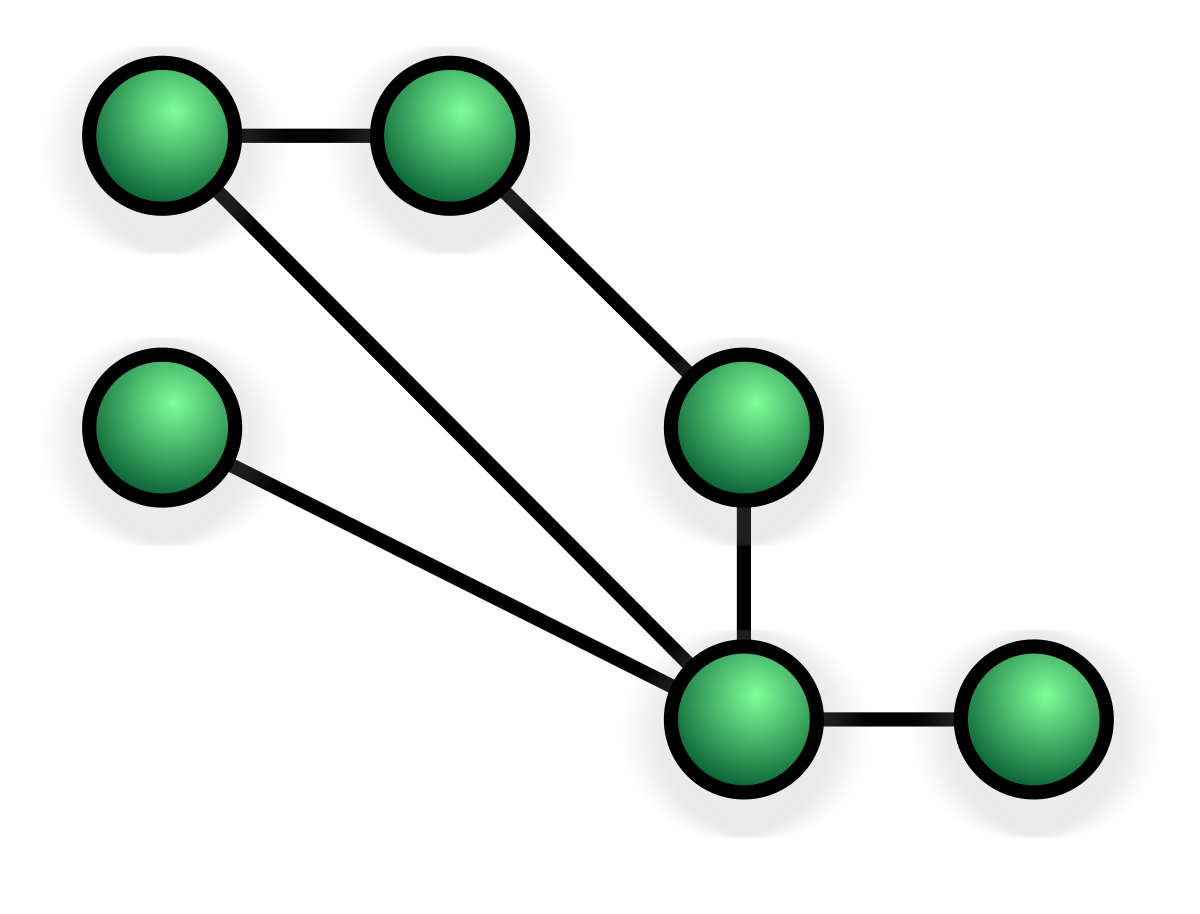
\includegraphics[scale=1]{mesh_partial}  
	\caption[Topologi Partially Connected Mesh]{Topologi Partially Connected Mesh} 
	\label{fig:mesh_partial} 
\end{figure} 
\begin{figure} [H]
	\centering  
	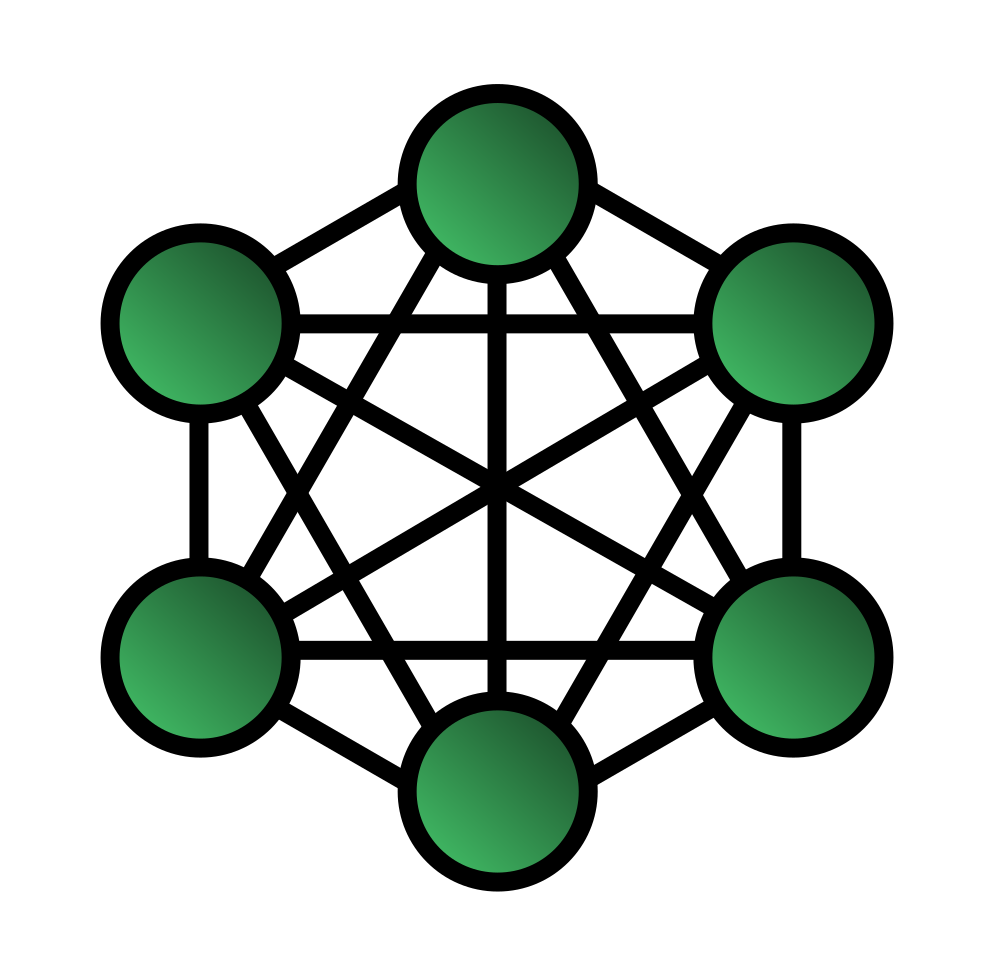
\includegraphics[scale=1]{mesh_fully}  
	\caption[Topologi Fully Connected Mesh]{Topologi Fully Connected Mesh} 
	\label{fig:mesh_fully} 
\end{figure} 

Arsitektur yang biasanya dipakai pada \textit{Wireless Sensor Network} adalah \textbf{arsitektur flat / peer-to-peer} dan \textbf{arsitektur hierarki}. Selain itu dalam membangun \textit{Wireless Sensor Network} perlu juga diperhatikan jalur komunikasi yang digunakan untuk menghubungkan antar \textit{sensor node} saat transfer data. Untuk area \textit{sensing} yang tidak terlalu luas dan hanya menggunakan sedikit \textit{sensor node} dapat menggunakan cara komunikasi \textbf{\textit{single hop}}. Sedangkan untuk daerah yang luas dan memerlukan banyak \textit{sensor node} dapat menggunakan cara komunikasi \textbf{\textit{multi hop}}. 

\begin{figure} [H]
	\centering  
	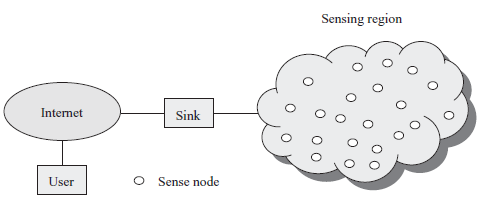
\includegraphics[scale=1]{arsitektur}  
	\caption[Arsitektur Wireless Sensor Network]{Arsitektur Wireless Sensor Network} 
	\label{fig:arsitektur} 
\end{figure} 

\subsubsection{Single-Hop dan Multi-Hop}
Untuk mengirim data ke sink node setiap sensor node dapat menggunakan single-hop long-distance transmission. Single-hop long-distance ini berarti setiap sensor node akan mengirimkan data ke sink node hanya satu kali lompatan walaupun jarak antara sink node dengan sensor node itu sangat jauh. Dalam jaringan sensor, penggunaan energi paling besar adalah saat melakukan komunikasi dibandingan saat sensing. Penggunaan energi akan semakin bertambah jika jarak sink dan sensor node semakin jauh. Untuk menangani masalah tersebut muncul protokol multi-hop.

Pada protokol multi-hop sensor node akan disusun saling berdekatan dan terhubung dengan yang lain. Jadi saat akan berkomunikasi dengan sink node, sensor node harus mengirimkan data tersebut ke sensor node tetangganya dan diteruskan hingga sampai ke sink node. Karena jarak yang saling berdekatan maka penggunaan energi dapat efektif. Single-hop dan multi-hop ini dapat digunakan dengan topologi flat maupun hierarki sesuai dengan kebutuhan sistem.

\subsubsection{Arsitektur Flat / Peer-to-Peer}
Pada arsitektur flat, setiap \textit{sensor node} memiliki peran atau \textit{role} yang sama dalam melakukan \textit{sensing}. Secara fungsional hanya terdapat dua macam \textit{sensor node} pada arsitektur flat, yaitu \textit{source node} dan \textit{sink node}. Karena jumlah \textit{sensor node} yang banyak maka tidak mungkin menentukan \textit{global identified} untuk setiap \textit{sensor node} pada jaringan ini. Untuk mendapatkan data dilakukan dengan cara \textit{sink node} melakukan pengiriman data ke semua \textit{sensor node} pada area \textit{sensing} dengan cara \textit{flooding} dan hanya \textit{sensor node} yang sesuai yang akan merespon \textit{sink node}. Setiap \textit{sensor node} mengirimkan data ke \textit{sink node} dengan \textit{multi hop} dan melalui node tetangganya yang terhubung dengannya untuk meneruskan data (Gambar~\ref{fig:flat}).
% gambar flat
\begin{figure} [H]
	\centering  
	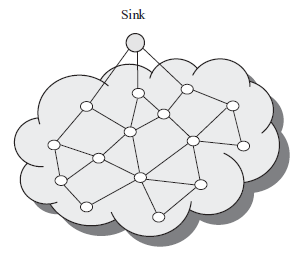
\includegraphics[scale=1]{flat}  
	\caption[Arsitektur flat pada \textit{Wireless Sensor Network}]{Arsitektur flat pada \textit{Wireless Sensor Network}} 
	\label{fig:flat} 
\end{figure} 

\subsubsection{Arsitektur Hierarki}
Pada arsitektur hierarki, semua sensor node dikelompokan ke dalam cluster-cluster. Terdapat cluster head pada setiap cluster. Cluster head ini yang mengumpulkan data dari setiap sensor node di bawahnya dan meneruskan data yang telah diterima ke base station atau sink. Hal yang perlu diperhatikan pada arsitektur hierarki adalah pemilihan sensor node sebagai cluster head dan sensor node yang melakukan sensing. Penggunaan energi yang paling besar dalam Wireless Sensor Network ini adalah saat melakukan komunikasi yaitu saat mengirimkan data ke sensor node lain. Maka untuk sensor node yang memiliki energi kecil dapat digunakan untuk sensing, karena sensor node sensing ini hanya melakukan komunikasi ke cluster head. Cluster head harus memiliki energi atau daya yang lebih banyak, karena cluster head akan bertugas menerima hasil sensing sensor node di bawahnya dan meneruskan data ke sink node. 

Masalah yang utama pada clustering ini adalah pemilihan cluster head dan bagaimana cara mengatur setiap cluster. Terdapat beberapa cara untuk membuat clustering ini. Bedasarkan jarak antara cluster head dengan cluster member, dapat dibuat clustering dengan single hop atau multi hop seperti pada Gambar~\ref{fig:cluster_single} dan Gambar~\ref{fig:cluster_multi}. Sedangkan jika berdasarkan jumlah tier dapat dibangun clustering single tier atau multi tier (Gambar~\ref{fig:cluster_multitier}).
\begin{figure} [H]
	\centering  
	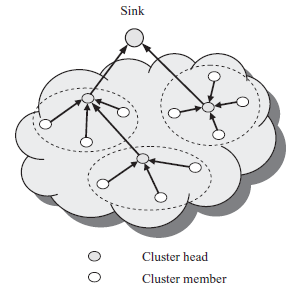
\includegraphics[scale=0.9]{cluster_single}  
	\caption[Arsitektur hierarki pada \textit{Wireless Sensor Network} dengan \textit{single hop} terhadap \textit{Cluster Head}]{Arsitektur hierarki pada \textit{Wireless Sensor Network} dengan \textit{single hop} terhadap \textit{Cluster Head}} 
	\label{fig:cluster_single} 
\end{figure} 
\begin{figure} [H]
	\centering  
	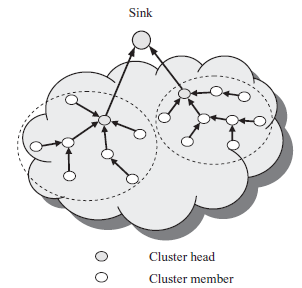
\includegraphics[scale=0.8]{cluster_multi}  
	\caption[Arsitektur hierarki pada \textit{Wireless Sensor Network} dengan \textit{multi hop}]{Arsitektur hierarki pada \textit{Wireless Sensor Network} dengan \textit{multi hop}} 
	\label{fig:cluster_multi} 
\end{figure} 
\begin{figure} [H]
	\centering  
	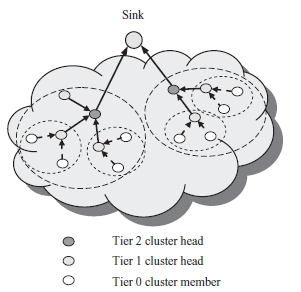
\includegraphics[scale=0.8]{cluster_multitier}  
	\caption[Clsutering dengan multi tier]{Clsutering dengan multi tier} 
	\label{fig:cluster_multitier} 
\end{figure}

%
\subsection{Layer pada Wireless Sensor Network}
Wireless Sensor Network memiliki lima layer protokol: physical layer, data link layer, network layer, transport layer, dan application layer, seperti pada Gambar~\ref{fig:layer}. 
\begin{figure} [H]
	\centering  
	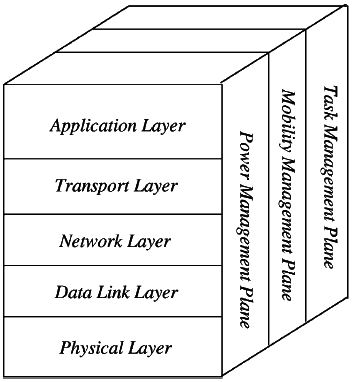
\includegraphics[scale=0.5]{layer}  
	\caption[Layer pada \textit{Wireless Sensor Network}]{Layer pada \textit{Wireless Sensor Network}} 
	\label{fig:layer} 
\end{figure} 

%00 wireless sensor network hal 293
\subsection{Sistem Operasi}
Setiap node sensor memerlukan sistem operasi (OS) untuk mengontrol perangkat keras dan perangkat lunak. Sistem operasi tradisional tidak dapat digunakan pada WSN. Pada sistem operasi tradisional digunakan untuk mengatur proses, memory, CPU time, dan file system. Terdapat beberapa hal yang harus ditangani oleh sistem operasi dalam WSN yaitu:
\begin{enumerate}
	\item WSN memerlukan real-time scheduler. Data yang didapat harus segera dikirim atau diproses.
	\item Pengaturan memori karena memory pada WSN sangat kecil.
	\item Pengaturan data yang efisien terkait dengan microprocessor dan memori yang terbatas
	\item Mendukung kode pemrograman yang efisien dan reliable karena dapat terjadi perubahan kode saat implementasi.
	\item Mendukung pengaturan sumber daya untuk menambah waktu hidup dari sensor node dan meningkatkan performa dengan sleep time atau wake up time saat terdapat interupsi dari lingkungan.
	\item Mendukung antarmuka untuk pemrograman dan antarmuka perangkat lunak. 
\end{enumerate}

Beberapa sistem operasi yang umum digunakan pada WSN antara lain :
\begin{enumerate}
	\item TinyOS
	\item Contiki
	\item LiteOS
\end{enumerate}

%Operating SYstem for WSN a survey - hal 7
\subsubsection{TinyOS}

%Operating SYstem for WSN a survey - hal 11
\subsubsection{Contiki}

%Operating SYstem for WSN a survey - hal 23
\subsubsection{LiteOS}



\section{Data Transfer pada Wireless Sensor Network} 
 
\section{Prinsip Reliable Data Transfer pada Wireless Sensor Network}
\label{sec:reliable}
Refrensi dari paper reliable. isinya link level retransmission, end to end retransmission, erasure code, Alternate Route (BVR) , dan route fix.
 
\section{Pengembangan Pemrograman pada Wireless Sensor Network}
\label{sec:pemrograman_wsn}


\newpage
\subsection{Tabel}  
Berikut adalah contoh pembuatan tabel. 
Penempatan tabel dan gambar secara umum diatur secara otomatis oleh \LaTeX{}, perhatikan contoh di file bab2.tex untuk melihat bagaimana cara memaksa tabel ditempatkan sesuai keinginan kita.

Perhatikan bawa berbeda dengan penempatan judul gambar gambar, keterangan tabel harus diletakkan di atas tabel!!
Lihat Tabel~\ref{tab:contoh1} berikut ini:

\begin{table}[H] %atau h saja untuk "kira kira di sini"
	\centering 
	\caption{Tabel contoh}
	\label{tab:contoh1}
	\begin{tabular}{cccc}
		\toprule
		& $v_{start}$ & $\mathcal{S}_{1}$ & $v_{end}$\\

		\midrule
		$\tau_{1}$ & 1 & 12& 20\\
		$\tau_{2}$ & 1 &  & 20\\
		$\tau_{3}$ & 1 & 9 & 20\\
		$\tau_{4}$ & 1 &  & 20\\

		\bottomrule
		
	\end{tabular} 
\end{table}
Tabel~\ref{tab:cthwarna1} dan Tabel~\ref{tab:cthwarna2} berikut ini adalah tabel dengan sel yang berwarna dan ada dua tabel yang bersebelahan. 
\begin{table}[H]
	\begin{minipage}[c]{0.49\linewidth}
		\centering
		\caption{Tabel bewarna(1)}
		\label{tab:cthwarna1}
		\begin{tabular}{ccccc}
			\toprule
			 & $v_{start}$ & $\mathcal{S}_{2}$ & $\mathcal{S}_{1}$ & $v_{end}$\\
			
			\midrule
			$\tau_{1}$ & 1 & 5 \cellcolor{green}& 12& 20\\
			$\tau_{2}$ & 1 & 8 \cellcolor{green}& & 20\\
			$\tau_{3}$ & 1 & 2/8/17 \cellcolor{green}& 9 & 20\\
			$\tau_{4}$ & 1 & \cellcolor{red}& & 20\\
			
			\bottomrule

		\end{tabular}
	\end{minipage}
	\begin{minipage}[c]{0.49\linewidth}
		
		\centering 
		\caption{Tabel bewarna(2)}
		\label{tab:cthwarna2}
		\begin{tabular}{ccccc}
			\toprule
			 & $v_{start}$ & $\mathcal{S}_{1}$ & $\mathcal{S}_{2}$ & $v_{end}$\\
			
			\midrule
			$\tau_{1}$ & 1 & 12& 5 \cellcolor{red} &20\\
			$\tau_{2}$ & 1 &  &  8 \cellcolor{green} &20\\
			$\tau_{3}$ & 1 & 9 & 2/8/17 \cellcolor{green} &20\\
			$\tau_{4}$ & 1 &   & \cellcolor{red} &20\\
			
			\bottomrule
		
		\end{tabular}
	\end{minipage}
\end{table}

 
\subsection{Kutipan}
\label{subs:kutipan} 
Berikut contoh kutipan dari berbagai sumber, untuk keterangan lebih lengkap, silahkan membaca file referensi.bib yang disediakan juga di template ini.
Contoh kutipan:
\begin{itemize}
	\item Buku:~\cite{berg:08:compgeom} 
	\item Bab dalam buku:~\cite{kreveld:04:GIS}
	\item Artikel dari Jurnal:~\cite{buchin:13:median}
	\item Artikel dari prosiding seminar/konferensi:~\cite{kreveld:11:median}
	\item Skripsi/Thesis/Disertasi:~\cite{lionov:02:animasi}~\cite{wiratma:10:following}~\cite{wiratma:22:later}
	\item Technical/Scientific Report:~\cite{kreveld:07:watertight}
	\item RFC (Request For Comments):~\cite{RFC1654}
	\item Technical Documentation/Technical Manual:~\cite{Z.500}~\cite{unicode:16:stdv9}~\cite{google:16:and7}
	\item Paten:~\cite{webb:12:comm}
	\item Tidak dipublikasikan:~\cite{wiratma:09:median}~\cite{lionov:11:cpoly}
	\item Laman web:~\cite{erickson:03:cgmodel}  
	\item Lain-lain:~\cite{agung:12:tango}
\end{itemize}    
  
\subsection{Gambar}

Pada hampir semua editor, penempatan gambar di dalam dokumen \LaTeX{} tidak dapat dilakukan melalui proses {\it drag and drop}.
Perhatikan contoh pada file bab2.tex untuk melihat bagaimana cara menempatkan gambar.
Beberapa hal yang harus diperhatikan pada saat menempatkan gambar:
\begin{itemize}
	\item Setiap gambar {\bf harus} diacu di dalam teks (gunakan {\it field} {\sc label})
	\item {\it Field} {\sc caption} digunakan untuk teks pengantar pada gambar. Terdapat dua bagian yaitu yang ada di antara tanda $[$ dan $]$ dan yang ada di antara tanda $\{$ dan $\}$. Yang pertama akan muncul di Daftar Gambar, sedangkan yang kedua akan muncul di teks pengantar gambar. Untuk skripsi ini, samakan isi keduanya.
	\item Jenis file yang dapat digunakan sebagai gambar cukup banyak, tetapi yang paling populer adalah tipe {\sc png} (lihat Gambar~\ref{fig:ularpng}), tipe {\sc jpg} (Gambar~\ref{fig:ularjpg}) dan tipe {\sc pdf} (Gambar~\ref{fig:ularpdf})
	\item Besarnya gambar dapat diatur dengan {\it field} {\sc scale}.
	\item Penempatan gambar diatur menggunakan {\it placement specifier} (di antara tanda  $[$ dan $]$ setelah deklarasi gambar.
	Yang umum digunakan adalah {\bf H} untuk menempatkan gambar {\bf sesuai} penempatannya di file .tex atau  {\bf h} yang berarti "kira-kira" di sini. \\
	Jika tidak menggunakan {\it placement specifier}, \LaTeX{} akan menempatkan gambar secara otomatis untuk menghindari bagian kosong pada dokumen anda.
	Walaupun cara ini sangat mudah, hindarkan terjadinya penempatan dua gambar secara berurutan. 	
	\begin{itemize}
		\item Gambar~\ref{fig:ularpng} ditempatkan di bagian atas halaman, walaupun penempatannya dilakukan setelah penulisan 3 paragraf setelah penjelasan ini.
		\item Gambar~\ref{fig:ularjpg} dengan skala 0.5 ditempatkan di antara dua buah paragraf. Perhatikan penulisannya di dalam file bab2.tex!
		\item Gambar~\ref{fig:ularpdf} ditempatkan menggunakan {\it specifier} {\bf h}.
	\end{itemize}
\end{itemize}
 
\dtext{17-18}
\begin{figure} 
	\centering  
	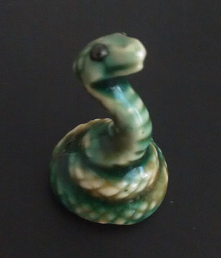
\includegraphics[scale=1]{ular-png}  
	\caption[Gambar {\it Serpentes} dalam format png]{Gambar {\it Serpentes} dalam format png} 
	\label{fig:ularpng} 
\end{figure} 

\dtext{19-20}
\begin{figure}[H]
	\centering  
	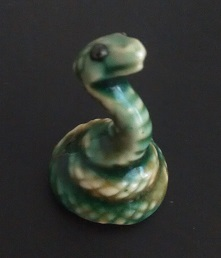
\includegraphics[scale=0.5]{ular-jpg}  
	\caption[Ular kecil]{Ular kecil} 
	\label{fig:ularjpg} 
\end{figure} 
\dtext{21-22}

\begin{figure}[ht] 
	\centering  
	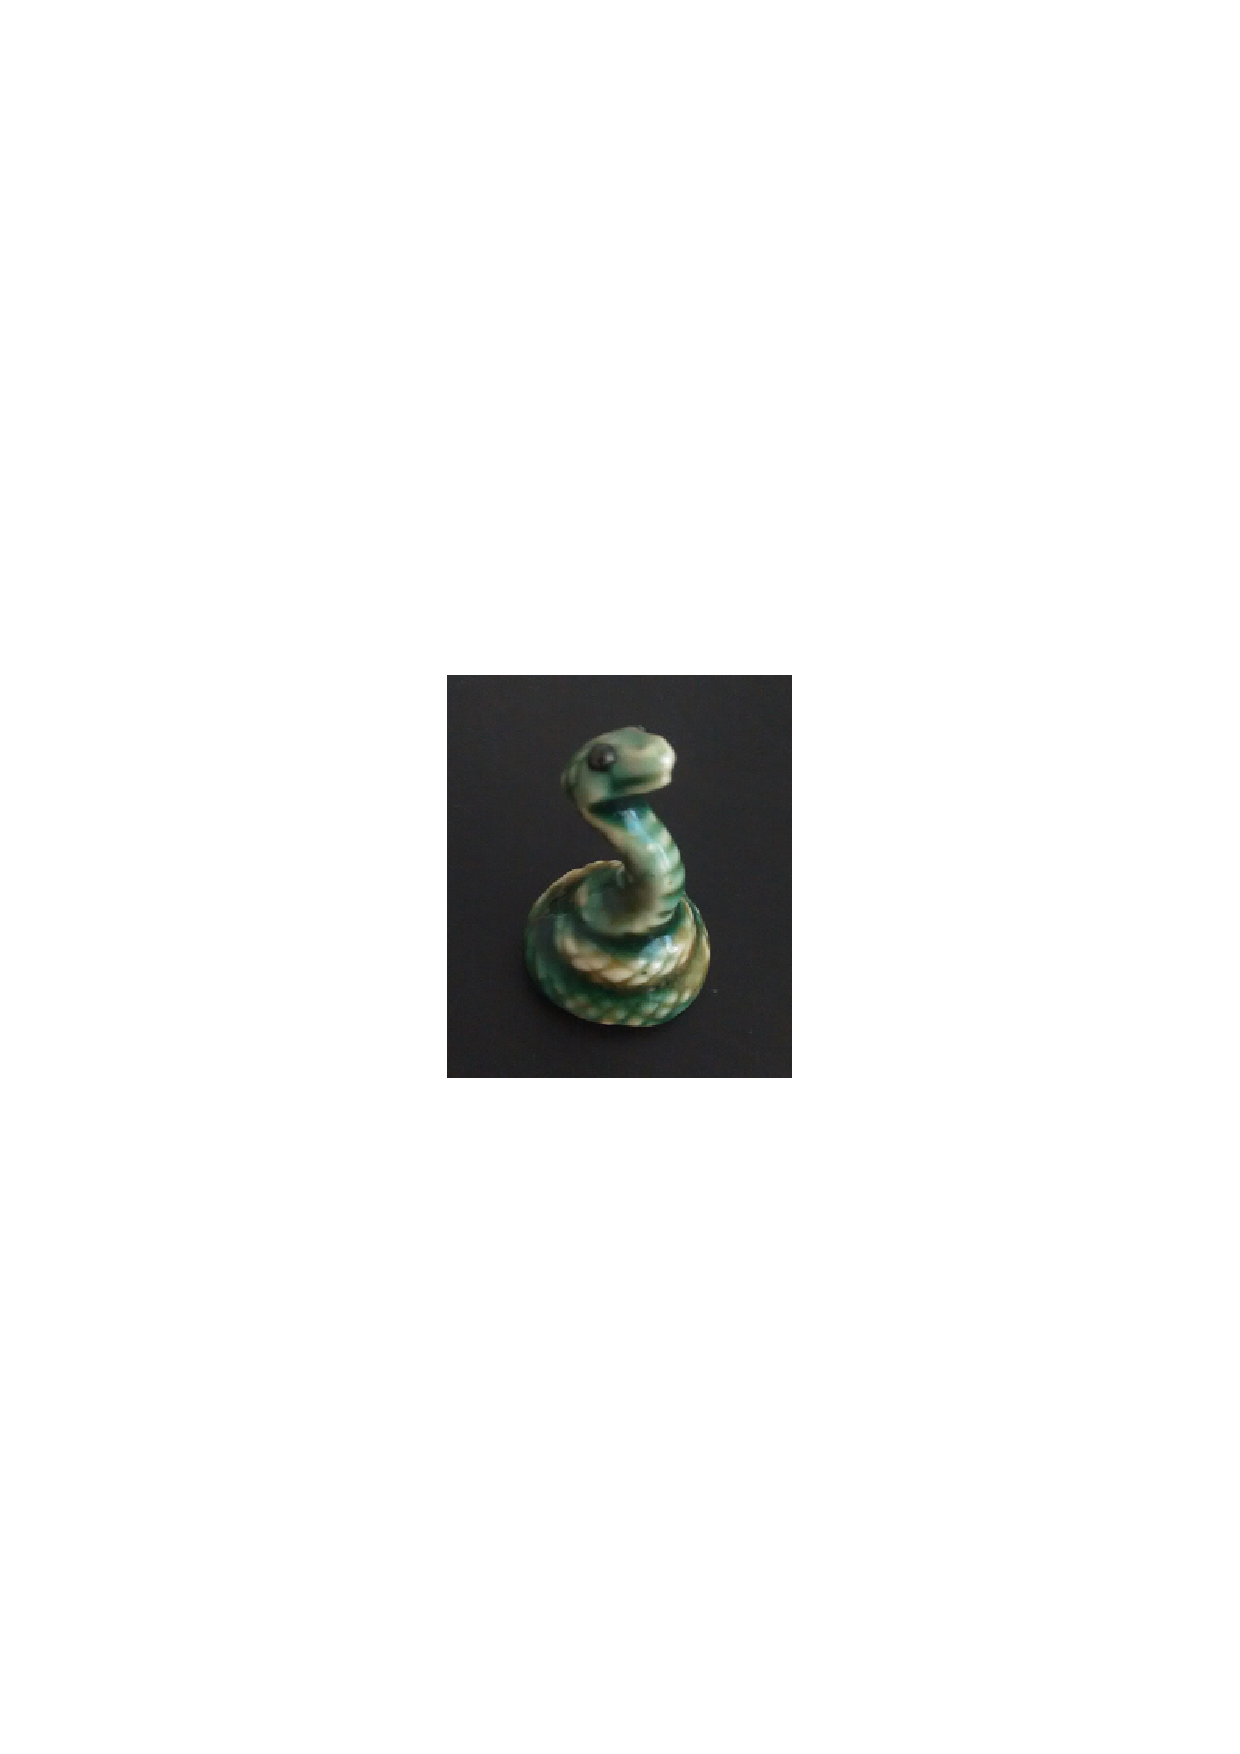
\includegraphics[scale=1]{ular-pdf}  
	\caption[ {\it Serpentes} betina]{ {\it Serpentes} jantan} 
	\label{fig:ularpdf} 
\end{figure} 
 
